%\documentclass[varwidth,border=10pt]{standalone}
\documentclass[aps,pra,twocolumn,superscriptaddress]{revtex4-1} %reprint
\thispagestyle{empty}
%\usepackage{subcaption}
%\usepackage[labelformat=parens,labelsep=quad, skip=3pt]{caption}
\usepackage{etex}
\usepackage{amsmath}
\usepackage{bm}
\usepackage{bbm}
\usepackage{listings}
% % \textwidth 16cm \textheight 23.5cm
% \renewcommand{\baselinestretch}{1.2}
\usepackage{graphicx}
\usepackage{graphics}
\usepackage{epsfig}
\usepackage{color}
\usepackage[dvipsnames]{xcolor}
\usepackage{multirow}
\usepackage[colorlinks]{hyperref}
\usepackage{fancyhdr}
\usepackage{calc}
\usepackage{natbib} %[numbers]
\usepackage{bibentry}
\usepackage{bbm}
\usepackage{bbold}

% todo list and commands
%\usepackage{todonotes}
%% to avoid the conflict with amths package % not working
%\makeatletter
%\providecommand\@dotsep{5}
%\makeatother
%\listoftodos\relax
%\usepackage{makeidx}
%\allowdisplaybreaks
%% for eps transfering to pdf.
%\usepackage[update,prepend]{epstopdf}
%\usepackage{ifpdf}
%
%\ifpdf
%   \usepackage{graphicx}
%   \usepackage{epstopdf}
%   \epstopdfsetup{suffix=}
%   \DeclareGraphicsRule{.eps}{pdf}{.pdf}{`epstopdf #1}
%   \pdfcompresslevel=9
%\else
%   \usepackage{graphicx}
%\fi
% subfig
\usepackage{mwe}
\usepackage[caption=false]{subfig}
% to fix a figure's position using [H] option of thec figure.
\usepackage{float}
% to use \lesssim and other math symbols
%\usepackage{amssymb}
% set package options
\captionsetup[subfloat]{position=top,singlelinecheck=off,labelfont={normalsize,sf}, %justification=raggedright,
  labelformat=simple,listofformat=subparens,aboveskip=0pt,parskip=0pt,farskip=5pt,
  captionskip=0pt}

% customize subfigure label to capitals
\renewcommand{\thesubfigure}{(\alph{subfigure})}
  
  %==== scattering and optical pumping rates ====%
  \newcommand{\gammauu}{\gamma_{\uparrow \rightarrow \uparrow}}
  \newcommand{\gammadd}{\gamma_{\downarrow \rightarrow \downarrow}}
  \newcommand{\gammaud}{\gamma_{\uparrow \rightarrow \downarrow}}
  \newcommand{\gammadu}{\gamma_{\downarrow \rightarrow \uparrow}}
  \newcommand{\gammau}{\gamma_{\uparrow}}
  \newcommand{\gammad}{\gamma_{\downarrow}}
  
  %==== effective areas ======
  \newcommand{\Ain}{A_{\rm in}}
  \newcommand{\Abir}{A_N}
  \newcommand{\AF}{A_{\rm Far}} % for the Faraday protocol.
  \newcommand{\Ai}{A_{\rm in}} % for the input light.
  \newcommand{\Aint}{A_{\rm int}} % for the interaction area.
  
\begin{document}
\begin{figure}[htb]
\centering
 \begin{minipage}[h]{0.99\linewidth}
 %\begin{tabular}{*{2}{b{0.2\textwidth-2\tabcolsep}}}
 \raisebox{3pt}{
  \subfloat[h][]{
    %% This file was created by matlab2tikz.
%
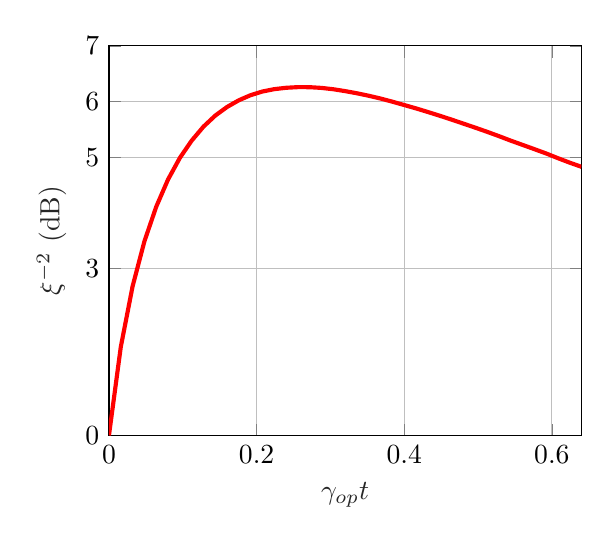
\begin{tikzpicture}

\begin{axis}[%
width=6cm,
height=4.948cm,
at={(0cm,0cm)},
scale only axis,
xmin=0.0000,
xmax=0.6400,
xlabel style={font=\color{white!15!black}},
xlabel={$\gamma_{op}t$},
ymin=0.0000,
ymax=7.0000,
ytick={0.0000,3.0000,5.0000,6.0000,7.0000,8.0000},
ylabel style={font=\color{white!15!black}},
ylabel={$\xi^{-2}$ (dB)},
axis background/.style={fill=white},
xmajorgrids,
ymajorgrids
]
\addplot [color=red, line width=1.5pt, forget plot]
  table[row sep=crcr]{%
0.0000	-0.0000\\
0.0160	1.5869\\
0.0320	2.6777\\
0.0480	3.4854\\
0.0640	4.1073\\
0.0800	4.5969\\
0.0960	4.9858\\
0.1120	5.2951\\
0.1280	5.5470\\
0.1440	5.7463\\
0.1600	5.9008\\
0.1760	6.0219\\
0.1920	6.1135\\
0.2080	6.1792\\
0.2240	6.2214\\
0.2400	6.2458\\
0.2560	6.2575\\
0.2720	6.2565\\
0.2880	6.2434\\
0.3040	6.2194\\
0.3200	6.1858\\
0.3360	6.1468\\
0.3520	6.1025\\
0.3680	6.0522\\
0.3840	5.9960\\
0.4160	5.8755\\
0.4320	5.8107\\
0.4480	5.7440\\
0.4640	5.6746\\
0.4960	5.5304\\
0.5121	5.4557\\
0.5281	5.3781\\
0.5441	5.2971\\
0.5761	5.1444\\
0.5921	5.0664\\
0.6081	4.9818\\
0.6241	4.9007\\
0.6401	4.8260\\
};
\end{axis}
\end{tikzpicture}%
    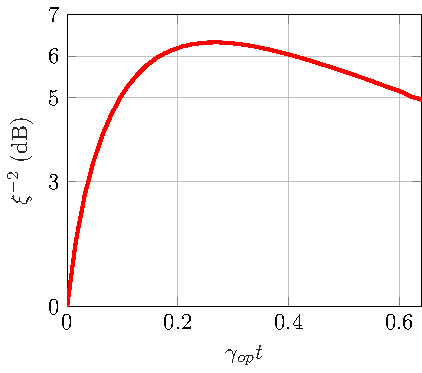
\includegraphics[width=0.45\linewidth]{../Fig6a}
    }}
    \hfill
  \subfloat[h][]{
      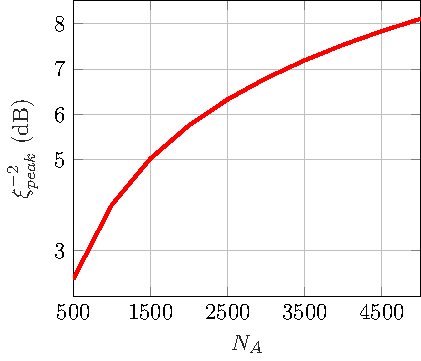
\includegraphics[width=0.45\linewidth]{../Fig6b}
      %% This file was created by matlab2tikz.
%
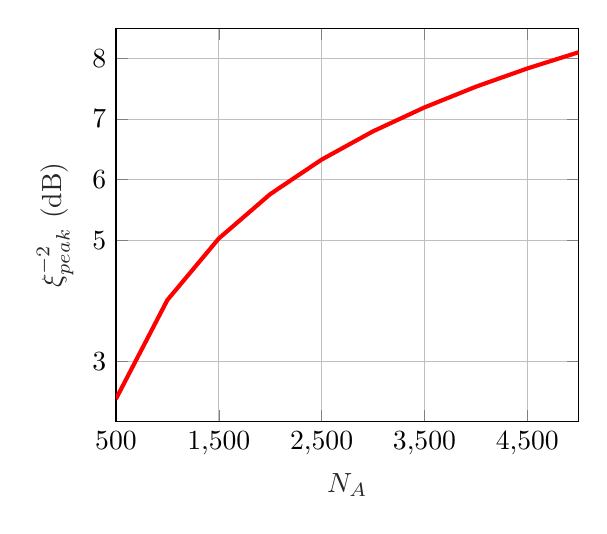
\begin{tikzpicture}

\begin{axis}[%
width=5.877cm,
height=5cm,
at={(0cm,0cm)},
scale only axis,
xmin=500.0000,
xmax=5000.0000,
xtick={500.0000,1500.0000,2500.0000,3500.0000,4500.0000},
xlabel style={font=\color{white!15!black}},
xlabel={$N_A$},
ymin=2.0000,
ymax=8.5000,
ytick={3.0000,5.0000,6.0000,7.0000,8.0000},
ylabel style={font=\color{white!15!black}},
ylabel={$\xi^{-2}_{peak}$ (dB)},
axis background/.style={fill=white},
xmajorgrids,
ymajorgrids
]
\addplot [color=red, line width=1.5pt, forget plot]
  table[row sep=crcr]{%
500.0000	2.3793\\
1000.0000	4.0121\\
1500.0000	5.0278\\
2000.0000	5.7605\\
2500.0000	6.3307\\
3000.0000	6.7978\\
3500.0000	7.1922\\
4000.0000	7.5342\\
4500.0000	7.8352\\
5000.0000	8.1036\\
};
\end{axis}
\end{tikzpicture}%
      }
   \end{minipage}\vfill
   \begin{minipage}[h]{0.99\linewidth}
    %\begin{tabular}{*{2}{b{0.2\textwidth-2\tabcolsep}}}
     \subfloat[h][]{
       %% This file was created by matlab2tikz.
%
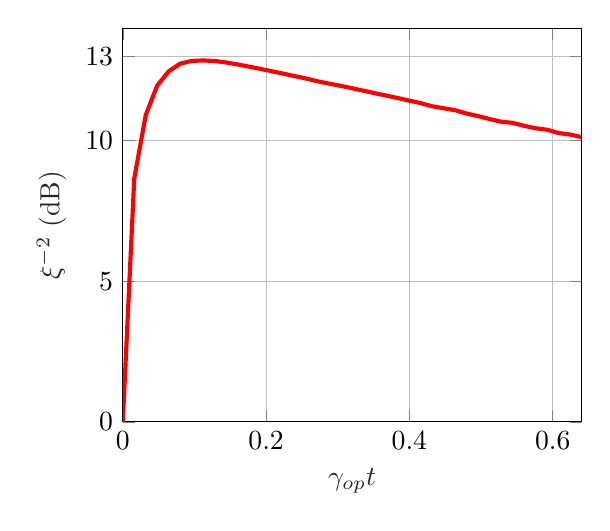
\begin{tikzpicture}

\begin{axis}[%
width=5.824cm,
height=5cm,
at={(0cm,0cm)},
scale only axis,
xmin=0.0000,
xmax=0.6400,
xlabel style={font=\color{white!15!black}},
xlabel={$\gamma_{op}t$},
ymin=-0.0000,
ymax=14.0000,
ytick={0.0000,5.0000,10.0000,13.0000,15.0000},
ylabel style={font=\color{white!15!black}},
ylabel={$\xi^{-2}$ (dB)},
axis background/.style={fill=white},
xmajorgrids,
ymajorgrids
]
\addplot [color=red, line width=1.5pt, forget plot]
  table[row sep=crcr]{%
0.0000	-0.0000\\
0.0160	8.6563\\
0.0320	10.9109\\
0.0480	11.9581\\
0.0640	12.4658\\
0.0800	12.7374\\
0.0960	12.8376\\
0.1120	12.8533\\
0.1280	12.8352\\
0.1440	12.7824\\
0.1600	12.7130\\
0.1760	12.6353\\
0.1920	12.5544\\
0.2240	12.3843\\
0.2400	12.2958\\
0.2560	12.2104\\
0.2720	12.1125\\
0.2880	12.0292\\
0.3040	11.9522\\
0.3360	11.7773\\
0.3520	11.6864\\
0.3680	11.6042\\
0.3840	11.5158\\
0.4000	11.4238\\
0.4160	11.3344\\
0.4320	11.2227\\
0.4640	11.0837\\
0.4800	10.9656\\
0.4960	10.8740\\
0.5121	10.7681\\
0.5281	10.6746\\
0.5441	10.6347\\
0.5601	10.5300\\
0.5761	10.4430\\
0.5921	10.3904\\
0.6081	10.2727\\
0.6241	10.2206\\
0.6401	10.1278\\
};
\end{axis}
\end{tikzpicture}%
       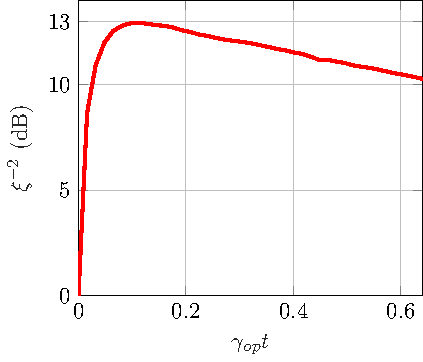
\includegraphics[width=0.45\linewidth]{../Fig6c}
       }
       \hfill
     \subfloat[h][]{
         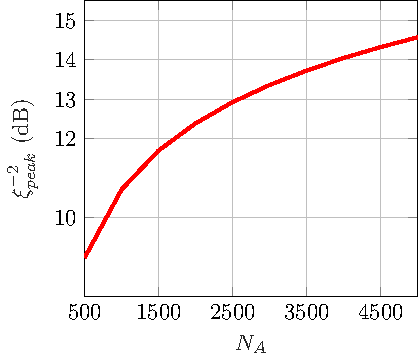
\includegraphics[width=0.45\linewidth]{../Fig6d}
         %% This file was created by matlab2tikz.
%
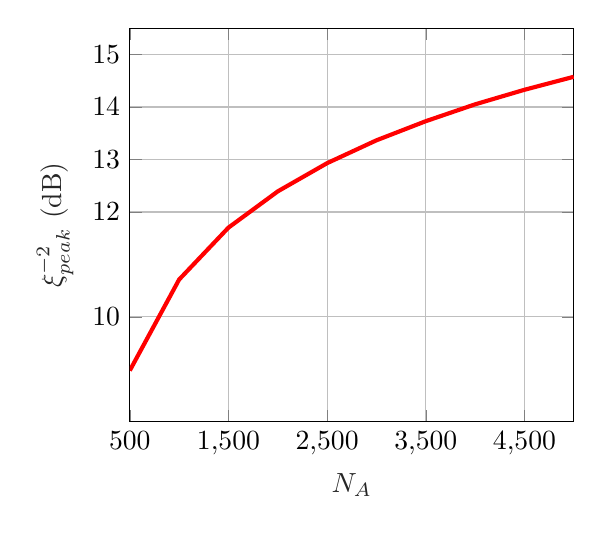
\begin{tikzpicture}

\begin{axis}[%
width=5.639cm,
height=5cm,
at={(0cm,0cm)},
scale only axis,
xmin=500.0000,
xmax=5000.0000,
xtick={500.0000,1500.0000,2500.0000,3500.0000,4500.0000},
xlabel style={font=\color{white!15!black}},
xlabel={$N_A$},
ymin=8.0000,
ymax=15.5000,
ytick={10.0000,12.0000,13.0000,14.0000,15.0000},
ylabel style={font=\color{white!15!black}},
ylabel={$\xi^{-2}_{peak}$ (dB)},
axis background/.style={fill=white},
xmajorgrids,
ymajorgrids
]
\addplot [color=red, line width=1.5pt, forget plot]
  table[row sep=crcr]{%
500.0000	8.9784\\
1000.0000	10.7121\\
1500.0000	11.7014\\
2000.0000	12.3921\\
2500.0000	12.9296\\
3000.0000	13.3648\\
3500.0000	13.7291\\
4000.0000	14.0500\\
4500.0000	14.3273\\
5000.0000	14.5751\\
};
\end{axis}
\end{tikzpicture}%
         }
   \end{minipage}
\end{figure}
\end{document}